\documentclass[12pt]{article}
\usepackage[utf8]{inputenc}
\usepackage[T1]{fontenc}
\usepackage{pdflscape} 
\usepackage{lmodern}
\usepackage[a4paper,bindingoffset=0.2in,%
            left=0.5in,right=0.5in,top=0.5in,bottom=1in,%
            footskip=.25in]{geometry}
\usepackage[colorlinks=true, linkcolor=Black, urlcolor=Blue]{hyperref}
\usepackage{graphicx}
\usepackage{subcaption}
\usepackage{listings}
\usepackage{color}
\usepackage[table]{xcolor}
\definecolor{lightgray}{gray}{0.9}

\definecolor{codegreen}{rgb}{0,0.6,0}
\definecolor{codegray}{rgb}{0.5,0.5,0.5}
\definecolor{codepurple}{rgb}{0.58,0,0.82}
\definecolor{backcolour}{rgb}{0.95,0.95,0.92}

\lstdefinestyle{mystyle}{
	backgroundcolor=\color{backcolour},   
	commentstyle=\color{codegreen},
	keywordstyle=\color{magenta},
	numberstyle=\tiny\color{codegray},
	stringstyle=\color{codepurple},
	basicstyle=\ttfamily\footnotesize,
	breakatwhitespace=false,         
	breaklines=true,                 
	captionpos=b,                    
	keepspaces=true,                 
	numbers=left,                    
	numbersep=5pt,                  
	showspaces=false,                
	showstringspaces=false,
	showtabs=false,                  
	tabsize=2
}


\begin{document}
\title{Sprawozdanie z zadania na Informatykę w Medycynie\\
\large Wykrywanie naczyń dna siatkówki oka\\
\large Sebastian Michoń 136770, Patryk Jedlikowski 136723}
\date{\vspace{-10ex}}
\maketitle

\section{Wstęp}
Dane są 3 różne notebooki
\begin {enumerate}
\item Basic\_version.ipynb - rozwiązanie na 3.0 - baseline model, wykorzystujący podstawowe techniki przetwarzania obrazów, w tym operacje morfologiczne.
\item kNN\_version.ipynb - rozwiązanie na 4.0 - wersja, która wykorzystuje podobieństwo (odleglość) obserwacji w zbiorze testowym do obserwacji ze zbioru treningowego celem przyporządkowania elementu ze zbioru testowego do odpowiedniej klasy. Skorzystano tutaj z wariancji kolorów i momentów centralnych
\item Random\_forest.ipynb - rozwiązanie na 5.0 - wersja używa podzbioru obserwacji do stworzenia pojedynczego drzewa - "silnego predyktora" (strong learner), po stworzeniu 50 takich drzew (które nie są ze sobą związane) i procesie trenowania ich używane są one do stwierdzenia, czy dany fragment obrazu jest naczyniem krwionośnym. Do Hyperparameter Tuningu (Znalezienie najlepszej maksymalnej wartości głębokości drzewa) użyta została k-krotna skrośna walidacja.
\end {enumerate}

\section{Model podstawowy}
\begin {enumerate}
	\item Wczytywany jest obraz w czerni i bieli (w kolejnych wersjach algorytmu - kNN i Random forest - to się zmieni)
	\item Wstępne przetwarzanie składa się z: normalizacji histogramu kolorów, denoisingu (który ma praktycznie zerowy wpływ na jakość predykcji) oraz 11-krotnego poddania obrazu wpływowi kernela Gaussa (blura, 5*5) - dzięki temu obraz jest dużo bardziej rozmyty, co ułatwi znalezienie tylko interesujących z perspektywy zadania krawędzi.
	\item Właściwe przetwarzanie obrazu to użycie filtra prewitta do wyróżnienia wszystkich krawędzi, które później, w końcowej fazie będę modyfikował.
	\item Końcowa faza przetwarzania to, kolejno:
	\begin{enumerate}
		\item Nałożenie zerodowanej maski obiektywu na powstały obraz: erozja rozszerzy czarną przestrzeń (obwódkę) maski obiektywu, następnie wykonana zostanie operacja logicznego \& na rozszerzonej masce i obrazie powstałym po użyciu filtra krawędziowego. Dzięki temu usunę z obrazu po filtrowaniu krawędzie na zetknięciu maski z właściwym obrazem.
		\item Usunięcie wykrytych krawędzi tam, gdzie obraz jest najjaśniejszy - dzięki temu usunę białą plamkę widoczną na każdym obrazie z końcowego efektu przetwarzania. Opiera się to na thresholdingu: usuwam krawędzie tam, gdzie stopień jasności jest wyższy niż \(\frac{2}{3}\) maksymalnej jasności obrazu (czyli wyższy niż 165).
		\item Dokonuję kolejno morfologicznego domknięcia i erozji obrazu. Dzięki temu grubość krawędzi na obrazie wynikowym zostanie zmniejszona, ponadto zostaną one wypełnione od wewnątrz.
	\end{enumerate}
	\item Do ewaluacji algorytmu użyto średniej geometrycznej miar: precision i recall. Średnia geometryczna była wygodniejsza od arytmetycznej, ponieważ mocniej zaniżała oszacowaną skuteczność algorytmu, jeśli jedno z recall/precision było bliskie 0. Dla 20 przetwestowanych obrazów z zestawu średnia średnich geometrycznych tych miar to 0.5729099817180116.
\end {enumerate}

\section{Klasyfikator odległościowy}
\begin{enumerate}
	\item Wczytywany jest obraz zarówno w czerni i bieli, jak i w kolorze
	\item Nie dokonano wstępnego przetwarzania, ponieważ nie prowadziło ono do zwiększenia skuteczności, wręcz przeciwnie - usunięcie normalizacji histogramu kolorów zwiększyło średnią geometryczną precision i recall o 0.05. Być może wynika to z większego rozrzutu miar przy zmianach histogramu przy stałym znaczeniu wariancji między kolorami dla całego dataseta, a co za tym idzie mniejszej użyteczności wariancji po skalowaniu obrazu.
	\item Aby wytrenować algorytm, wybrany został podzbiór punktów jednego obrazu. Podzbiór był wybierany w taki sposób, że:
	\begin{enumerate}
		\item Losuję koordynaty \(x, y\) pojedynczego punkt z obrazu.
		\item Jeśli koordynaty te należą do punktu, który nie został jeszcze wybrany i nie należy do maski i albo jest naczyniem krwionośnym, albo losowo wybrana liczba całkowita z przedziału \(x \in <0;3>: x \equiv 0\ (mod\ 4)\) to zostaje dodany do zbioru wybranych punktów. Dzięki temu liczba wybranych punktów z obu klas jest bardziej zrównoważona, bo na 10 wylosowanych par liczb około jedna reprezentuje naczynie krwionośne, a ten algorytm zwiększa tą liczbę. Oczywiście dla zbioru testowego nie używam kategoryzacji na naczynia krwionośne i resztę - wyniku używam dopiero do ewaluacji skuteczności. W innym przypadku zaniżałbym liczbę false negatives, zwiększając tym samym kluczowy z perspektywy oceny skuteczności recall.
		
		\item Dla każdego punktu z wybranego zbioru punktów znajdowana jest informacja o nim, w tym: intensywność kolorów w punkcie, wariancje kolorów w obrazie o rozmiarze 10*10, którego centrum jest ten punkt (używany jest padding zerami, aby każdy podobraz, włącznie z tymi na brzegach obrazu mógł uzyskać takie informacje), a także jego momenty centralne, wartość koloru w punkcie na czarno-białym obrazie (aby móc odsiać białą plamkę) i informacja, czy wokół punktu jest zetknięcie dwóch płaszczyzn maski obiektywu - aby odsiać krawędzie nie będące naczyniami krwionośnymi wokół maski obiektywu. Nie używałem momentów Hu, ponieważ spowalniały one proces predykcji nie zwiększając skuteczności algorytmu.
		\item Dla wybranego zbioru punktów znajdowana jest także informacja o wartośći maski eksperckiej (z naczyniami krwionośnymi) w tym punkcie - dla zbioru treningowego do trenowania algorytmu, dla testowego do estymacji jego skuteczności.
		\item Przed treningiem dokonana zostaje normalizacja zbioru testowego i treningowego - bez niej algorytm osiąga takie same rezultaty, ale proces trenowania i predykcji wykonuje się około 10 razy wolniej. Wagi dla poszczególnych zmiennych są takie same (uniform).
		\item Algorytm jest trenowany na wybranych danych  z 3 obrazów, po 40000 różnych punktów z każdego. Testowanie dla pojedynczego obrazu także odbywa się z udziałem 40000 punktów
	\end{enumerate}
	\item Analogicznie wybierany jest zbiór informacji do testowanego obrazu. W ramach testowania tak samo jak w poprzednim rozwiązaniu porównywany jest rezultat treningu z maską ekspercką. Rezultaty są niższe o około 0.11 dla średniej geometrycznej w stosunku do tych z zadania poprzedniego, zmniejsza się także accuracy - które nie używa w tym algorytmie punktów spoza maski obiektywu. Punkty z maski zawsze były klasyfikowane jako true negative, co nie ma wpływu ani na precision, ani recall, tylko na accuracy.
\end{enumerate}


\section{Las drzew losowych}
\begin{enumerate}
	\item Proces wstępnego przetwarzania (czyli jego brak) i wybór punktów jednego obrazu jest analogiczny do kNN-a. Różnicą jest występowanie hyperparameter tuningu używającego k-krotnej skrośnej walidacji i ternary searcha, a także proces treningu.
	\item Trening odbywa się na wybranych punktach z 3 różnych obrazów, ręcznie wybranych, które były relatywnie niepodobne do siebie - to dało możliwość lepszego pokrycia zbioru testowego. W treningu pokryto 600.000 punktów z 3 obrazów (\(3*\frac{1}{40}\) obrazka), te obrazy później miały najwyższe średnie geometryczne i accuracy w trakcie testowania - wartość średniej geometrycznej wynosiła około 0.65-0.74, accuracy 0.95. Ponadto zaprzestano równoważenia zbioru treningowego w kontekście klas, bo to nie wpływało pozytywnie na jakość tego algorytmu.
	\item K-skrośna walidacja została użyta do hyperparameter tuningu: z wybranego zestawu treningowego wyodrębniane są losowo 4 zbiory, następnie dla danych \(a, b\) 4 lasy są trenowane na 3 grupach i testowane na 4., każdy las testowany na innej z 4 grup. \(a, b\) oznaczają maksymalną głębokość drzewa: zakładane jest, że zależność precyzji drzewa od głębokości jest najpierw niemalejąca (im większa głębokość, tym wyższa precyzja - drzewo o głębokości 2 uchwyci więcej informacji niż drzewo o głębokości 1), następnie nierosnąca (im większa głębokość, tym większa złożoność pamięciowa i tym więcej zbędnych informacji zapamiętuje drzewo - gdyby nie operowanie na lesie, a nie pojedynczym drzewie, niechybnie zaszedłby overfitting). To daje podstawy do użycia ternary searcha - szukam dla przedziału \(<l;r>\) możliwych wartości maksymalnej głębokości wartości maksymalizującej średnią średnich geometrycznych recall i precision na zbiorach testowych. Wartość ta będzie użyta jako hiperparametr w ostatecznym trenowaniu algorytmu na całym zbiorze treningowym. Poszukuję jej tak:
	\begin{enumerate}
		\item znajduję \(a=\lfloor\frac{r}{3}\rfloor, b=\lfloor\frac{2*r}{3}\rfloor\)
		\item Jeśli wartość funkcji \(f\) (średnia średnich geometrycznych) jest większa dla \(f(a)\) - to znaczy, że funkcja maleje już gdzieś na przedziale \(<a;b>\), a zatem osiąga supremum w przedziale \(<0;b>\) - przypisuję zatem \(r=b\)
		\item Analogicznie, dla \(f(b)>f(a)\) funkcja rośnie gdzieś na przedziale \(<a;b>\), a zatem osiąga supremum w przedziale \(<a;r>\) - przypisuję zatem \(l=a\)
		\item Jeśli \(f(a)=f(b)\), to supremum musi leżeć pomiędzy nimi - przypisuję \(l=a, r=b\)
	\end{enumerate}
\end{enumerate}




\section{Tablica wynków}
Oznaczenia i skróty:
\begin{enumerate}
	\item title - nazwa obrazka
	\item tp - True positive - liczba takich rezultatów w wybranym podzbiorze
	\item tn - True negative
	\item fp - False positive
	\item fn - False negative
	\item acc - Accuracy = \(\frac{tp+tn}{tp+tn+fp+fn}\)
	\item prec - Precision = \(\frac{tp}{tp+fp}\)
	\item rec - Recall = \(\frac{tp}{tp+fn}\)
	\item sgeom - średnia geometryczna rec i prec: \(\sqrt{rec*prec}\)
\end{enumerate}
W ostatniej linijce tablicy algorytmu umieszczono średnie wyliczanych parametrów.
\begin{flushleft}
\begin{landscape}
		\captionof{table}{Efektywność poszczególnych algorytmów: Random Forest bez preprocessingu. Pogrubiono obrazy dane na zbiorze treningowym}
		\begin{tabular}{| l | l | l | l | l | l | l | l | l |}
			\rowcolor{gray!50}
			\hline
			title & tp & tn & fp & fn & acc & prec & rec & sgeom \\ \hline
			\textbf{RFC-01\_dr} & 6204 & 186538 & 5976 & 1283 & 0.9637 & 0.8286 & 0.5094 & 0.6497 \\ \hline
			RFC-02\_dr & 6247 & 180672 & 8819 & 4263 & 0.9346 & 0.5944 & 0.4146 & 0.4964 \\ \hline
			RFC-03\_dr & 4871 & 181496 & 9575 & 4059 & 0.9318 & 0.5455 & 0.3372 & 0.4289 \\ \hline
			RFC-04\_dr & 3496 & 183237 & 9814 & 3454 & 0.9337 & 0.5030 & 0.2627 & 0.3635 \\ \hline
			RFC-05\_dr & 12091 & 101481 & 2851 & 83578 & 0.5679 & 0.1264 & 0.8092 & 0.3198 \\ \hline
			RFC-06\_dr & 14173 & 103494 & 3752 & 78582 & 0.5883 & 0.1528 & 0.7907 & 0.3476 \\ \hline
			RFC-07\_dr & 9181 & 177662 & 9162 & 3996 & 0.9342 & 0.6967 & 0.5005 & 0.5905 \\ \hline
			\textbf{RFC-08\_dr} & 11053 & 180594 & 6866 & 1488 & 0.9582 & 0.8813 & 0.6168 & 0.7373 \\ \hline
			RFC-09\_dr & 14940 & 11829 & 1037 & 172195 & 0.1338 & 0.0798 & 0.9351 & 0.2732 \\ \hline
			RFC-10\_dr & 11718 & 167469 & 9229 & 11585 & 0.8959 & 0.5029 & 0.5594 & 0.5304 \\ \hline
			RFC-11\_dr & 14505 & 159607 & 5738 & 20151 & 0.8706 & 0.4185 & 0.7165 & 0.5476 \\ \hline
			\textbf{RFC-12\_dr} & 8341 & 182453 & 7788 & 1419 & 0.9540 & 0.8546 & 0.5171 & 0.6648 \\ \hline
			RFC-13\_dr & 4974 & 181989 & 11250 & 1788 & 0.9348 & 0.7356 & 0.3066 & 0.4749 \\ \hline
			RFC-14\_dr & 9412 & 177742 & 8556 & 4291 & 0.9358 & 0.6869 & 0.5238 & 0.5998 \\ \hline
			RFC-01\_h & 18471 & 99702 & 5413 & 76415 & 0.5909 & 0.1947 & 0.7734 & 0.3880 \\ \hline
			RFC-02\_h & 15813 & 158602 & 7551 & 18035 & 0.8721 & 0.4672 & 0.6768 & 0.5623 \\ \hline
			RFC-03\_h & 21357 & 31084 & 3554 & 144006 & 0.2622 & 0.1292 & 0.8573 & 0.3328 \\ \hline
			RFC-04\_h & 19172 & 29259 & 2921 & 148649 & 0.2422 & 0.1142 & 0.8678 & 0.3149 \\ \hline
			RFC-05\_h & 7913 & 175137 & 13449 & 3502 & 0.9152 & 0.6932 & 0.3704 & 0.5067 \\ \hline
			RFC-06\_h & 11401 & 169258 & 12829 & 6513 & 0.9033 & 0.6364 & 0.4705 & 0.5472 \\ \hline
			\textbf{RFC-ALL} & 0 & 0 & 0 & 0 & 0.7662 & 0.4921 & 0.5908 & \textbf{0.4838}\\ \hline
	\end{tabular}
\end{landscape}
\end{flushleft}

	\begin{landscape}
		\captionof{table}{Efektywność poszczególnych algorytmów: kNN bez preprocessingu. Pogrubiono obrazy dane na zbiorze treningowym}
		\begin{tabular}{| l | l | l | l | l | l | l | l | l |}
			\rowcolor{gray!50}
			\hline
			title & tp & tn & fp & fn & acc & prec & rec & sgeom \\ \hline
			\textbf{kNN-01\_dr} & 1281 & 36302 & 1046 & 1372 & 0.9396 & 0.4828 & 0.5505 & 0.5156 \\ \hline
			kNN-02\_dr & 1502 & 35273 & 1567 & 1659 & 0.9194 & 0.4752 & 0.4894 & 0.4822 \\ \hline
			kNN-03\_dr & 767 & 36344 & 2125 & 765 & 0.9278 & 0.5007 & 0.2652 & 0.3644 \\ \hline
			kNN-04\_dr & 1133 & 35736 & 1634 & 1498 & 0.9217 & 0.4306 & 0.4095 & 0.4199 \\ \hline
			kNN-05\_dr & 2241 & 31646 & 620 & 5494 & 0.8472 & 0.2897 & 0.7833 & 0.4764 \\ \hline
			kNN-06\_dr & 2494 & 29520 & 1046 & 6941 & 0.8003 & 0.2643 & 0.7045 & 0.4315 \\ \hline
			kNN-07\_dr & 1867 & 34594 & 1700 & 1840 & 0.9115 & 0.5036 & 0.5234 & 0.5134 \\ \hline
			kNN-08\_dr & 924 & 35613 & 2679 & 785 & 0.9134 & 0.5407 & 0.2565 & 0.3724 \\ \hline
			kNN-09\_dr & 333 & 36439 & 2884 & 345 & 0.9193 & 0.4912 & 0.1035 & 0.2255 \\ \hline
			\textbf{kNN-10\_dr} & 2498 & 33478 & 1708 & 2317 & 0.8994 & 0.5188 & 0.5939 & 0.5551 \\ \hline
			kNN-11\_dr & 2610 & 33391 & 1365 & 2635 & 0.9000 & 0.4976 & 0.6566 & 0.5716 \\ \hline
			kNN-12\_dr & 558 & 36266 & 2655 & 522 & 0.9206 & 0.5167 & 0.1737 & 0.2995 \\ \hline
			kNN-13\_dr & 587 & 36243 & 2590 & 581 & 0.9207 & 0.5026 & 0.1848 & 0.3047 \\ \hline
			kNN-14\_dr & 947 & 35477 & 2686 & 891 & 0.9106 & 0.5152 & 0.2607 & 0.3665 \\ \hline
			kNN-01\_h & 3291 & 33010 & 1619 & 2081 & 0.9075 & 0.6126 & 0.6703 & 0.6408 \\ \hline
			\textbf{kNN-02\_h} & 3342 & 33855 & 1288 & 1516 & 0.9299 & 0.6879 & 0.7218 & 0.7047 \\ \hline
			kNN-03\_h & 4081 & 20177 & 859 & 14884 & 0.6064 & 0.2152 & 0.8261 & 0.4216 \\ \hline
			kNN-04\_h & 3980 & 21491 & 554 & 13976 & 0.6368 & 0.2217 & 0.8778 & 0.4411 \\ \hline
			kNN-05\_h & 1688 & 35051 & 2667 & 595 & 0.9185 & 0.7394 & 0.3876 & 0.5353 \\ \hline
			kNN-06\_h & 2712 & 34004 & 2167 & 1118 & 0.9179 & 0.7081 & 0.5559 & 0.6274 \\ \hline
			\textbf{kNN-ALL} & 0 & 0 & 0 & 0 & 0.8784 & 0.4857 & 0.4997 & \textbf{0.4635}\\ \hline
		\end{tabular}
	\end{landscape}

	\begin{landscape}
		\captionof{table}{Efektywność poszczególnych algorytmów: Image processing}
		\begin{tabular}{| l | l | l | l | l | l | l | l | l |}
			\rowcolor{gray!50}
			\hline
			title & tp & tn & fp & fn & acc & prec & rec & sgeom \\ \hline
			Proc-01\_dr & 305250 & 7460420 & 111032 & 308642 & 0.9487 & 0.4972 & 0.7333 & 0.6038 \\ \hline
			Proc-02\_dr & 342994 & 7292673 & 178884 & 370793 & 0.9328 & 0.4805 & 0.6572 & 0.5620 \\ \hline
			Proc-03\_dr & 267790 & 7150689 & 226610 & 540255 & 0.9063 & 0.3314 & 0.5416 & 0.4237 \\ \hline
			Proc-04\_dr & 318585 & 6729966 & 143594 & 993199 & 0.8611 & 0.2429 & 0.6893 & 0.4092 \\ \hline
			Proc-05\_dr & 367518 & 7374879 & 141460 & 301487 & 0.9459 & 0.5494 & 0.7221 & 0.6298 \\ \hline
			Proc-06\_dr & 357308 & 7115321 & 260658 & 452057 & 0.9129 & 0.4415 & 0.5782 & 0.5052 \\ \hline
			Proc-07\_dr & 508672 & 6931136 & 127687 & 617849 & 0.9089 & 0.4515 & 0.7993 & 0.6008 \\ \hline
			Proc-08\_dr & 404988 & 7166842 & 210789 & 402725 & 0.9250 & 0.5014 & 0.6577 & 0.5743 \\ \hline
			Proc-09\_dr & 219287 & 7525484 & 335160 & 105413 & 0.9462 & 0.6754 & 0.3955 & 0.5168 \\ \hline
			Proc-10\_dr & 511777 & 7055860 & 203112 & 414595 & 0.9245 & 0.5525 & 0.7159 & 0.6289 \\ \hline
			Proc-11\_dr & 476029 & 7165393 & 216908 & 327014 & 0.9335 & 0.5928 & 0.6870 & 0.6381 \\ \hline
			Proc-12\_dr & 332399 & 7180235 & 224325 & 448385 & 0.9178 & 0.4257 & 0.5971 & 0.5042 \\ \hline
			Proc-13\_dr & 363293 & 7330776 & 196186 & 295089 & 0.9400 & 0.5518 & 0.6493 & 0.5986 \\ \hline
			Proc-14\_dr & 452117 & 6875380 & 172819 & 685028 & 0.8952 & 0.3976 & 0.7235 & 0.5363 \\ \hline
			Proc-01\_h & 535643 & 6877202 & 298245 & 474254 & 0.9056 & 0.5304 & 0.6423 & 0.5837 \\ \hline
			Proc-02\_h & 580357 & 6516935 & 228081 & 859971 & 0.8671 & 0.4029 & 0.7179 & 0.5378 \\ \hline
			Proc-03\_h & 494976 & 7020955 & 369195 & 300218 & 0.9182 & 0.6225 & 0.5728 & 0.5971 \\ \hline
			Proc-04\_h & 526077 & 6993019 & 245524 & 420724 & 0.9186 & 0.5556 & 0.6818 & 0.6155 \\ \hline
			Proc-05\_h & 458840 & 7310816 & 279946 & 135742 & 0.9492 & 0.7717 & 0.6211 & 0.6923 \\ \hline
			Proc-06\_h & 611006 & 7048768 & 218864 & 306706 & 0.9358 & 0.6658 & 0.7363 & 0.7001 \\ \hline
			
			\textbf{Proc-ALL} & 0 & 0 & 0 & 0 & 0.9197 & 0.5120 & 0.6560 & \textbf{0.5729}\\ \hline
		\end{tabular}
	\end{landscape}

\begin{figure}[h!]
	\centering
	\begin{subfigure}[b]{0.99\linewidth}
		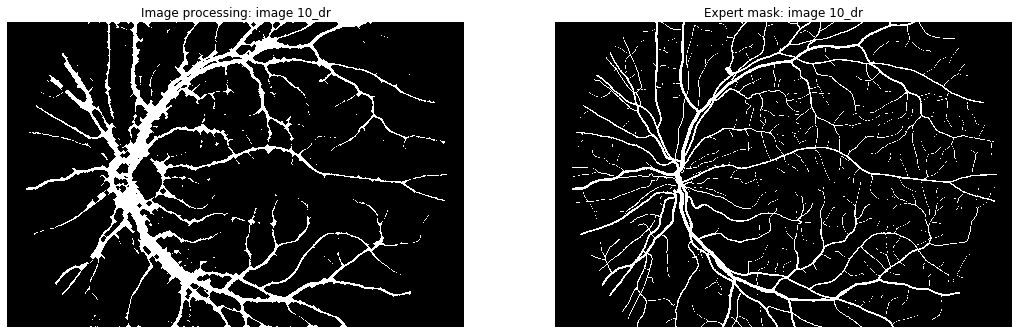
\includegraphics[width=\linewidth]{Results/process.png}
	\end{subfigure}
	\caption{Pełny obrazek poddany standardowemu przetwarzaniu obrazu - więcej przykładów w notebooku jupytera}
\end{figure}
\begin{figure}[h!]
	\begin{subfigure}[b]{0.98\linewidth}
		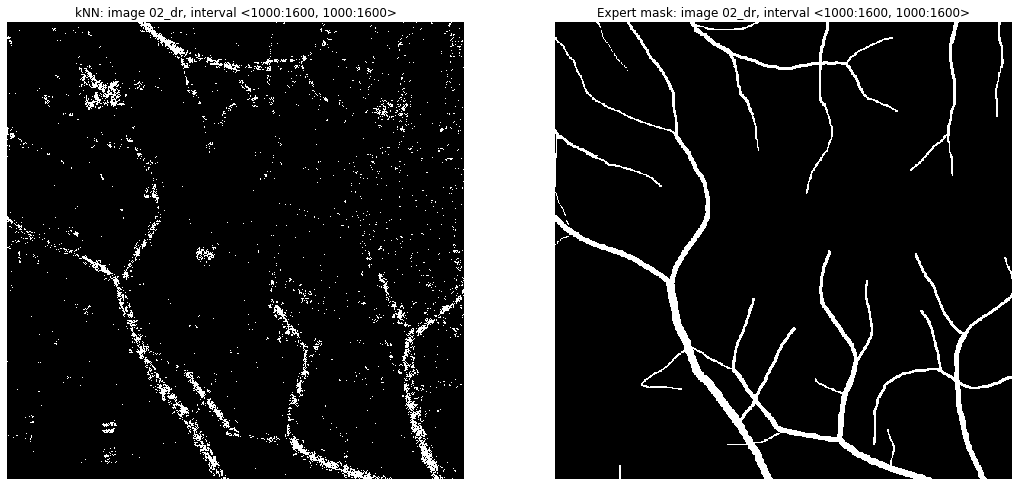
\includegraphics[width=\linewidth]{Results/kNN.png}
	\end{subfigure}
	\caption{Przykład działania algorytmu kNN - z lewej efekt kNN, z prawej maska ekspercka}
\end{figure}
\begin{figure}[h!]
	\begin{subfigure}[b]{0.98\linewidth}
		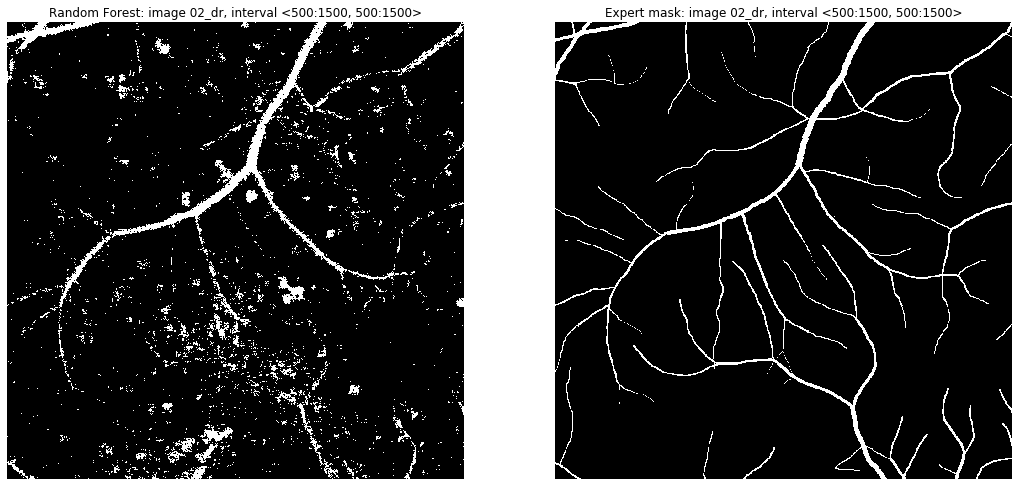
\includegraphics[width=\linewidth]{Results/rfc.png}
	\end{subfigure}
	\caption{Przykład działania algorytmu Random Forest - z lewej efekt lasu, z prawej maska ekspercka}
\end{figure}
\newpage
\section{Wnioski}
\begin{enumerate}
	\item Proste rozwiązanie oparte na manualnym przetwarzaniu obrazu osiągnęło satysfakcjonującą skuteczność o średniej geometrycznej rzędu 0.58. 
	
	\item Rozwiązanie oparte na lesie drzew decyzyjnych działa bardzo dobrze na danych, których podzbiór (choćby rzędu \(\frac{1}{200}\)) był dany na treningu algorytmu. W takich przypadkach rozwiązanie spisywało się lepiej niż każdy inny model. W pozostałych przypadkach nie funkcjonowało tak dobrze - wynika to zapewne z różnorodności danych, w szczególności związanych z dodatkowymi plamkami na obrazach. Problemu tego nie rozwiązuje, a być może nawet pogłębia normalizacja.
	
	\item Rozwiązanie oparte na k-tym najbliższym sąsiedzie działało przeciętnie nawet na danych, które widziało, natomiast było dużo bardziej odporne na dane odstające, wcześniej niewidziane - accuracy nigdy nie spadło poniżej 0.6, czego nie można powiedzieć o lesie drzew decyzyjnych.
	
	\item Aby algorytmy te działały lepiej, należałoby albo uzyskać lepsze dane, albo trenować na dużo większym zestawie treningowym. Dotyczy to w mniejszym stopniu kNN-a niż losowego lasu, który zależy tylko i wyłącznie od ilości danych zwizanych z obrazami, które testuje. Lasy drzew losowych rzadko są używane do image processingu, ponieważ po przekroczeniu pewnej ilości informacji właściwie nie są w stanie się nauczyć nowych wzorców, w przeciwieństwie do sieci neuronowych. Nie dało się tego zauważyć w tym projekcie, ponieważ operowano na bardzo małym zbiorze treningowym, przez co las losowy nie pokazał pełni swoich możliwości.
\end{enumerate}


\end{document}
